\documentclass[tikz]{standalone}
\usepackage{pgfplots}
\pgfplotsset{compat=1.15}
\usepackage{mathrsfs}
\usetikzlibrary{arrows,calc}
\usepackage{tkz-euclide}

\pagestyle{empty}

\definecolor{AngleClr}{rgb}{0,0.39215686274509803,0}
\definecolor{ShapeClr}{rgb}{0.6,0.2,0}

\begin{document}

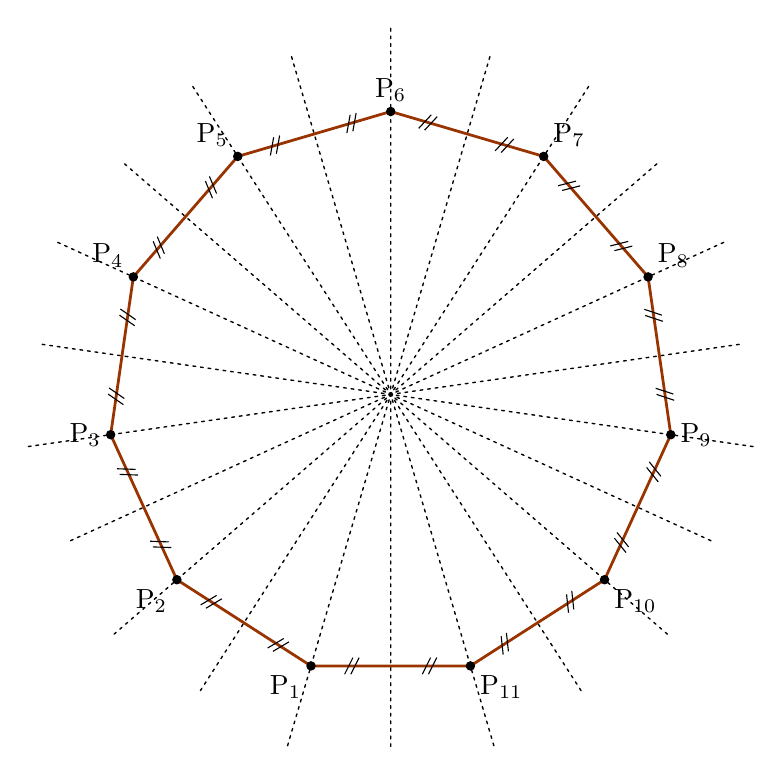
\begin{tikzpicture}[scale=.75]
\tkzSetUpLine[line width=1pt,color=black]
\tkzSetUpPoint[fill=black]

\tkzDefPoints{0/0/P0,2.7/0/P1}
\tkzDefRegPolygon[side,sides=11](P0,P1)

\tkzDefMidPoint(P1,P2) \tkzGetPoint{M1}
\tkzDefMidPoint(P2,P3) \tkzGetPoint{M2}
\tkzDefMidPoint(P3,P4) \tkzGetPoint{M3}
\tkzDefMidPoint(P4,P5) \tkzGetPoint{M4}
\tkzDefMidPoint(P5,P6) \tkzGetPoint{M5}
\tkzDefMidPoint(P6,P7) \tkzGetPoint{M6}
\tkzDefMidPoint(P7,P8) \tkzGetPoint{M7}
\tkzDefMidPoint(P8,P9) \tkzGetPoint{M8}
\tkzDefMidPoint(P9,P10) \tkzGetPoint{M9}
\tkzDefMidPoint(P10,P11) \tkzGetPoint{M10}
\tkzDefMidPoint(P11,P1) \tkzGetPoint{M11}

\tkzFillPolygon[fill=white](P1,P2,P3,P4,P5,P6,P7,P8,P9,P10,P11)

\tkzDrawSegments[line width=0.5pt,color=black,dashed,dash pattern=on 1pt off 1.75pt,add=0.15 and 0.15](P1,M6 P2,M7 P3,M8 P4,M9 P5,M10 P6,M11 P7,M1 P8,M2 P9,M3 P10,M4 P11,M5)


\tkzDrawPolygon[color=ShapeClr](P1,P2,P3,P4,P5,P6,P7,P8,P9,P10,P11)

\tkzDrawPoints[size=3](P1,P2,P3,P4,P5,P6,P7,P8,P9,P10,P11)
\tkzLabelPoint[below left](P1){${\rm P}_1$}
\tkzLabelPoint[below right](P2){${\rm P}_{11}$}
\tkzLabelPoint[below right](P3){${\rm P}_{10}$}
\tkzLabelPoint[right](P4){${\rm P}_9$}
\tkzLabelPoint[above right](P5){${\rm P}_8$}
\tkzLabelPoint[above right](P6){${\rm P}_7$}
\tkzLabelPoint[above](P7){${\rm P}_6$}
\tkzLabelPoint[above left](P8){${\rm P}_5$}
\tkzLabelPoint[above left](P9){${\rm P}_4$}
\tkzLabelPoint[left](P10){${\rm P}_3$}
\tkzLabelPoint[below left](P11){${\rm P}_2$}

\tkzMarkSegments[mark=s||,size=3](P1,M1 P2,M1 P2,M2 P3,M2 P3,M3 P4,M3 P4,M4 M4,P5 P5,M5 M5,P6 P6,M6 M6,P7 P7,M7 M7,P8 P8,M8 M8,P9 P9,M9 M9,P10 P10,M10 M10,P11 P11,M11 M11,P1)

\end{tikzpicture}

\end{document}
